\documentclass{article}
\usepackage[utf8]{inputenc}
\usepackage{amsmath}

\usepackage{graphicx}

\usepackage{utp-doc}


\usepackage{xcolor}
\usepackage{tikz}
\usepackage{pifont}
\usepackage{geometry}
\usepackage{float}
\usepackage{setspace}




% Configuración de página
%\geometry{a4paper, margin=2.5cm}
%\renewcommand{\familydefault}{\sfdefault}

% Colores institucionales
%\definecolor{UTPGreen}{HTML}{00833D}
%\definecolor{UTPGray}{HTML}{666666}

% Configuración de encabezados
%\pagestyle{fancy}
%\fancyhf{}
%\rhead{\thepage}
%\lhead{\textcolor{UTPGray}{\small AD.04.01.01 - Ciclos Termodinámicos}}


%\begin{document}
\begin{document}
	
	% Establecer espaciado entre líneas a 1.5
	\onehalfspacing
	
	%
	% --- Título de la Lectura ---
	\practicatitle{AD.04.01.01: Lectura de Ciclos Termodinámicos}
	
	% --- Metadatos de la Actividad ---
	\textbf{Asignatura:} Termodinámica Automotriz \\
	\textbf{Unidad IV:} - Sistemas y Ciclos de Potencia de Gas
	
	\vspace{5mm}
	\hrule
	\vspace{5mm}

% --- Portada ---
%\begin{center}
%    {\LARGE\textbf{\textcolor{UTPGreen}{UNIVERSIDAD TECNOLÓGICA DE PUEBLA}}}\\[0.5cm]
%    {\large\textbf{Actividad de Desarrollo}}\\[0.3cm]
%    {\Large\textbf{AD.04.01.01: Lectura de Ciclos Termodinámicos}}\\[0.5cm]
    
%    \textbf{Asignatura:} Termodinámica Automotriz \\
%    \textbf{Unidad IV:} Sistemas y Ciclos de Potencia de Gas\\[0.5cm]
    
    \hrule
%\end{center}

\vspace{1cm}

    % --- Contenido ---
    \tableofcontents
    \newpage

    \section{Introducción}

    Los \hl{ciclos termodinámicos de potencia} constituyen la base fundamental para comprender el funcionamiento de las \hl{máquinas térmicas} que convierten \hl{energía térmica} en \hl{trabajo mecánico}. Estos ciclos son secuencias ordenadas de \hl{procesos termodinámicos} que el \hl{fluido de trabajo} experimenta de manera cíclica para generar trabajo útil.

    En el contexto de la \hl{ingeniería automotriz}, el estudio de estos ciclos es esencial para el \hl{diseño}, \hl{análisis} y \hl{optimización} de \hl{motores de combustión interna}. Los \hl{ciclos ideales} nos proporcionan \hl{modelos teóricos} que, aunque no son perfectamente realizables en la práctica, nos permiten establecer \hl{límites de rendimiento} y comprender los \hl{principios físicos} que gobiernan el funcionamiento de los motores reales.

    Según Çengel y Boles (2015), las \hl{máquinas térmicas} se diseñan con el propósito de convertir \hl{energía térmica} en trabajo, y su desempeño se expresa en términos de la \hl{eficiencia térmica} ($\eta_{ter}$), que representa la relación entre el \hl{trabajo neto producido} y la \hl{entrada total de calor}.

    En esta lectura estudiaremos los \hl{ciclos fundamentales}: \hl{Carnot}, \hl{Otto} y \hl{Diesel}, analizando sus características, aplicaciones y limitaciones para proporcionar una base sólida en el análisis de \hl{sistemas de potencia automotrices}.

    \section{Desarrollo}

    \subsection{Fundamentos de los ciclos de potencia}

    Las \hl{máquinas térmicas} son dispositivos cíclicos donde el \hl{fluido de trabajo} regresa a su estado inicial al final de cada ciclo. Durante una parte del ciclo, el fluido realiza trabajo, y durante otra, se hace trabajo sobre el fluido. La diferencia entre estos dos trabajos constituye el \hl{trabajo neto} que entrega la máquina térmica (Moran et al., 2018).

    La \hl{eficiencia térmica} de cualquier máquina térmica se define como:

    \begin{equation}
    \eta_{ter} = \frac{W_{neto}}{Q_{entrada}} \quad \text{o} \quad \eta_{ter} = \frac{w_{neto}}{q_{entrada}}
    \end{equation}

    Donde:
    \begin{itemize}
        \item $W_{neto}$: Trabajo neto producido por ciclo (kJ)
        \item $Q_{entrada}$: Calor total suministrado por ciclo (kJ)
        \item $w_{neto}$, $q_{entrada}$: Valores específicos por unidad de masa (kJ/kg)
    \end{itemize}

    \subsubsection{Idealizaciones para ciclos de potencia}

    Para el análisis de \textbf{ciclos de potencia ideales}, se emplean las siguientes \textbf{simplificaciones}:

    \begin{enumerate}
        \item \textbf{Ausencia de fricción}: El fluido de trabajo no experimenta caídas de presión cuando fluye por tuberías o intercambiadores de calor.
        \item \textbf{Procesos de cuasiequilibrio}: Todos los procesos de expansión y compresión ocurren de manera \textbf{cuasiestática}.
        \item \textbf{Sistemas adiabáticos}: Las tuberías que conectan los componentes están perfectamente aisladas.
        \item \textbf{Desprecio de energías cinética y potencial}: Los cambios en estas energías son insignificantes comparados con los términos de trabajo y calor.
    \end{enumerate}

    \subsubsection{Diagramas termodinámicos}

    En los \textbf{diagramas P-v} y \textbf{T-s}, el \textbf{área encerrada} por las curvas del proceso representa el \textbf{trabajo neto producido} durante el ciclo, que también equivale a la \textbf{transferencia neta de calor}. El \textbf{diagrama T-s} es particularmente útil, ya que:

    \begin{itemize}
        \item El \textbf{área bajo la curva} del proceso representa la \textbf{transferencia de calor} para ese proceso específico.
        \item Un \textbf{proceso de adición de calor} avanza en dirección de \textbf{entropía creciente}.
        \item Un \textbf{proceso de rechazo de calor} avanza en dirección de \textbf{entropía decreciente}.
        \item Un \hl{proceso isentrópico} (adiabático reversible) avanza a \textbf{entropía constante}.
    \end{itemize}

    \begin{figure}[H]
        \centering
        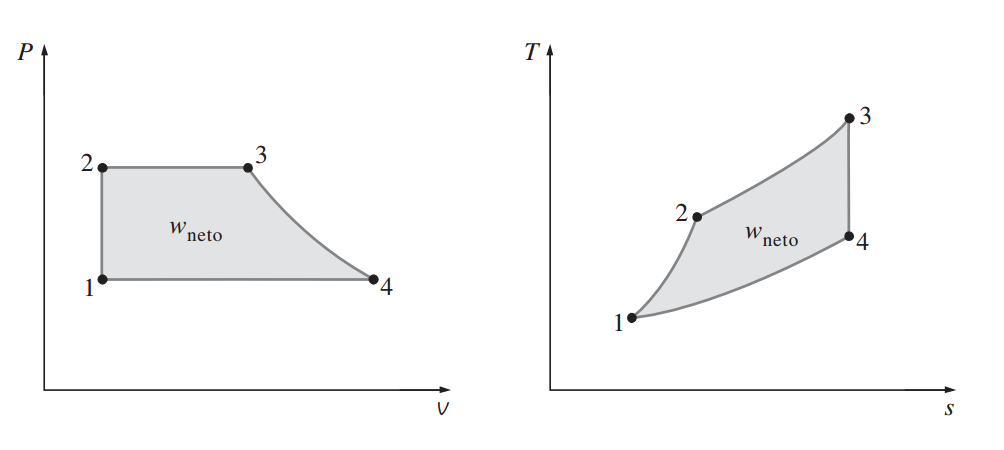
\includegraphics[width=0.8\textwidth]{Pasted_image_20250803091726.png}
        \caption{Diagramas P-v y T-s genéricos.}
        \label{fig:diagramas_genericos}
    \end{figure}

    \subsection{El ciclo de Carnot: el límite teórico de eficiencia}

    El \hl{ciclo de Carnot}, propuesto en 1824 por el ingeniero francés \textbf{Sadi Carnot}, representa el \textbf{ciclo termodinámico ideal} más eficiente posible entre dos \textbf{reservorios térmicos} a temperaturas constantes. Este ciclo establece el \textbf{límite teórico superior} de eficiencia para cualquier \hl{máquina térmica} que opere entre las mismas temperaturas, constituyendo el \textbf{estándar de referencia} contra el cual se comparan todos los ciclos reales (Çengel \& Boles, 2015).

    La \textbf{máquina térmica de Carnot} es completamente \hl{reversible}, lo que significa que todos sus procesos pueden invertirse sin dejar rastro en los alrededores. Esta característica la convierte en la máquina térmica más eficiente teóricamente posible.

    \subsubsection{Procesos del ciclo de Carnot}

    El \hl{ciclo de Carnot} consta de cuatro \textbf{procesos reversibles}:

    \paragraph{Proceso 1-2: Expansión Isotérmica Reversible}
    El \textbf{fluido de trabajo} se encuentra inicialmente a temperatura $T_H$ en contacto con una \textbf{fuente térmica} de alta temperatura. El gas se expande lentamente realizando \hl{trabajo} sobre los alrededores mientras mantiene su temperatura constante.

    \textbf{Ecuación del calor absorbido:}
    \begin{equation}
    Q_H = T_H \Delta S_{12}
    \end{equation}

    \paragraph{Proceso 2-3: Expansión Adiabática Reversible}
    Se elimina la fuente térmica y se aísla el sistema. El fluido continúa expandiéndose sin \textbf{intercambio de calor}, realizando trabajo mientras su temperatura disminuye de $T_H$ a $T_L$.

    \textbf{Relación temperatura-volumen:}
    \begin{equation}
    T_2 V_2^{\gamma-1} = T_3 V_3^{\gamma-1}
    \end{equation}

    \paragraph{Proceso 3-4: Compresión Isotérmica Reversible}
    El sistema se pone en contacto con un \textbf{sumidero térmico} a temperatura $T_L$. Una fuerza externa comprime el gas mientras este \textbf{cede calor} al sumidero, manteniendo su temperatura constante en $T_L$.

    \textbf{Ecuación del calor cedido:}
    \begin{equation}
    Q_L = T_L \Delta S_{34}
    \end{equation}

    \paragraph{Proceso 4-1: Compresión Adiabática Reversible}
    Se retira el sumidero térmico y se aísla nuevamente el sistema. El gas se comprime \textbf{adiabáticamente} hasta retornar a su estado inicial.

    \textbf{Relación temperatura-volumen:}
    \begin{equation}
    T_4 V_4^{\gamma-1} = T_1 V_1^{\gamma-1}
    \end{equation}

    \subsubsection{Eficiencia del Ciclo de Carnot}

    La \hl{eficiencia térmica} de cualquier máquina térmica se define como:

    \begin{equation}
    \eta_{ter} = \frac{W_{neto}}{Q_{entrada}} = 1 - \frac{Q_L}{Q_H}
    \end{equation}

    Para \textbf{máquinas térmicas reversibles}, la relación de transferencias de calor puede reemplazarse por la relación de \textbf{temperaturas absolutas}:

    \begin{equation}
    \left(\frac{Q_H}{Q_L}\right)_{rev} = \frac{T_H}{T_L}
    \end{equation}

    Por lo tanto, la \textbf{eficiencia del ciclo de Carnot} se expresa como:

    \begin{equation}
    \eta_{Carnot} = \eta_{ter,rev} = 1 - \frac{T_L}{T_H}
    \end{equation}

    Donde:
    \begin{itemize}
        \item $T_L$: Temperatura absoluta del \textbf{sumidero térmico} (K)
        \item $T_H$: Temperatura absoluta de la \textbf{fuente térmica} (K)
    \end{itemize}

    \begin{figure}[H]
        \centering
        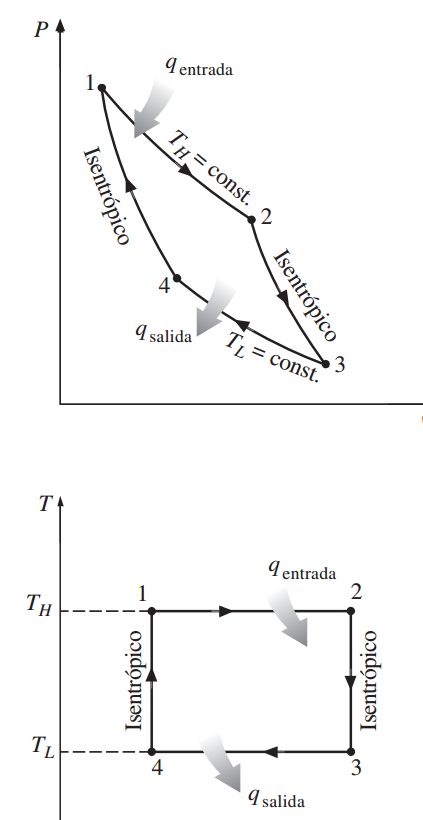
\includegraphics[width=0.7\textwidth]{Pasted_image_20250803092250.png}
        \caption{Ciclo de Carnot en diagramas P-v y T-s}
        \label{fig:carnot}
    \end{figure}

    \subsubsection{Principios de Carnot}

    Los \textbf{principios de Carnot} establecen dos conclusiones fundamentales:

    \begin{enumerate}
        \item La eficiencia de una máquina térmica irreversible es siempre menor que la eficiencia de una máquina reversible que opera entre los mismos reservorios.
        \item Las eficiencias de todas las máquinas térmicas reversibles que operan entre los mismos reservorios son \textbf{idénticas}.
    \end{enumerate}

    Estos principios pueden expresarse matemáticamente como:

    \begin{equation}
    \eta_{ter} \begin{cases}
    < \eta_{ter,rev} & \text{(máquina irreversible)} \\
    = \eta_{ter,rev} & \text{(máquina reversible)} \\
    > \eta_{ter,rev} & \text{(máquina imposible)}
    \end{cases}
    \end{equation}

    \subsection{El ciclo de Otto: motores de encendido por chispa}

    El \hl{ciclo de Otto}, nombrado en honor a \textbf{Nikolaus A. Otto} quien construyó exitosamente una máquina de cuatro tiempos en 1876, constituye el \textbf{modelo termodinámico ideal} para los \textbf{motores de encendido por chispa} (motores de gasolina). Este ciclo representa una \textbf{versión idealizada} del funcionamiento real de los \textbf{motores de combustión interna} de cuatro tiempos.

    \subsubsection{Funcionamiento del motor de cuatro tiempos}

    En los \textbf{motores reales}, el pistón ejecuta cuatro carreras completas (dos ciclos mecánicos) dentro del cilindro, mientras el cigüeñal completa dos revoluciones por cada \textbf{ciclo termodinámico}. Las cuatro carreras son:

    \begin{enumerate}
        \item \textbf{Carrera de admisión}: Entrada de la mezcla aire-combustible
        \item \textbf{Carrera de compresión}: Compresión de la mezcla
        \item \textbf{Carrera de potencia}: Combustión y expansión de gases
        \item \textbf{Carrera de escape}: Expulsión de gases de combustión
    \end{enumerate}

    \begin{figure}[H]
        \centering
        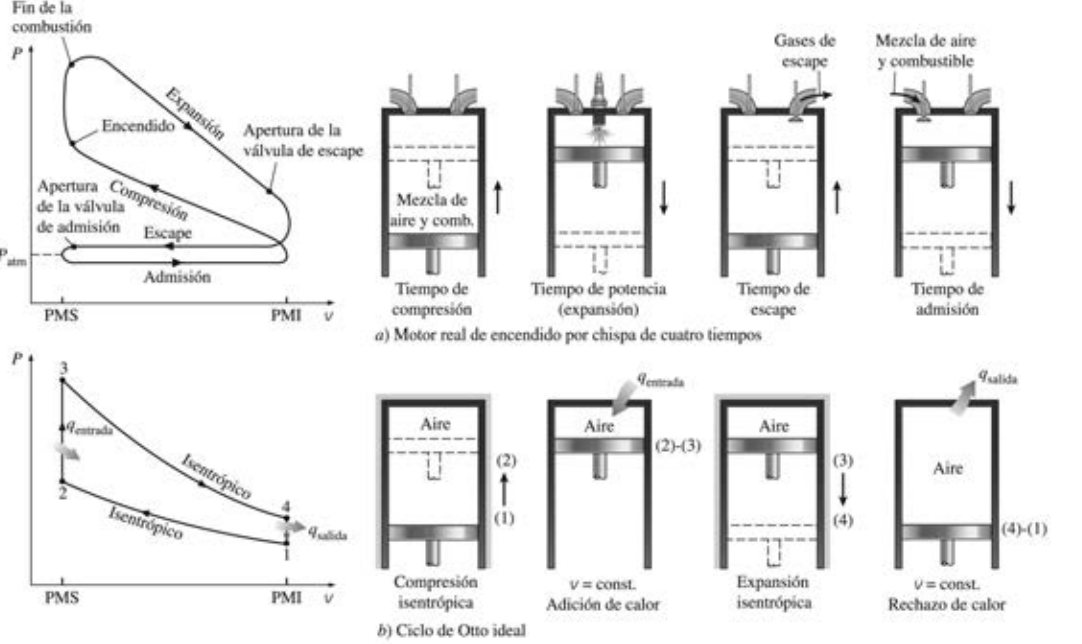
\includegraphics[width=0.9\textwidth]{Pasted_image_20250803092813.png}
        \caption{Motor de cuatro tiempos y ciclos Otto real e ideal}
        \label{fig:motor_otto}
    \end{figure}

    \subsubsection{Procesos del ciclo de Otto ideal}

    El \textbf{ciclo de Otto ideal} se compone de cuatro \textbf{procesos internamente reversibles}:

    \paragraph{Proceso 1-2: Compresión Isentrópica}
    La mezcla \textbf{aire-combustible} se comprime \textbf{adiabáticamente} desde el \textbf{punto muerto inferior} (\textbf{PMI}) hasta el \textbf{punto muerto superior} (\textbf{PMS}).

    \textbf{Relación de compresión:}
    $$
        r = \frac{V_1}{V_2} = \frac{V_{max}}{V_{min}}
    $$

    Para un \hl{proceso isentrópico} (adiabático reversible) en un \textbf{gas ideal}, las relaciones entre propiedades están gobernadas por el \textbf{índice adiabático} o \textbf{relación de calores específicos} ($\gamma$):

    \begin{equation}
    \gamma = \frac{c_p}{c_v}
    \end{equation}

    Donde:
    \begin{itemize}
        \item $c_p$: Calor específico a \textbf{presión constante} (kJ/kg·K)
        \item $c_v$: Calor específico a \textbf{volumen constante} (kJ/kg·K)
        \item $\gamma \approx 1.4$ para aire a temperatura ambiente
    \end{itemize}

    \textbf{Relaciones isentrópicas:}
    \begin{align}
    \frac{T_2}{T_1} &= \left(\frac{V_1}{V_2}\right)^{\gamma-1} = r^{\gamma-1} \\
    \frac{P_2}{P_1} &= \left(\frac{V_1}{V_2}\right)^{\gamma} = r^{\gamma}
    \end{align}

    \paragraph{Proceso 2-3: Adición de Calor a Volumen Constante}
    Este proceso simula la \textbf{combustión instantánea} de la mezcla. Se añade calor ($Q_H$) al sistema manteniendo el \textbf{volumen constante}.

    \textbf{Calor añadido:}
    \begin{equation}
    Q_H = m c_v (T_3 - T_2)
    \end{equation}

    \paragraph{Proceso 3-4: Expansión Isentrópica}
    Los \textbf{gases calientes} a alta presión se expanden \textbf{adiabáticamente}, empujando el pistón desde el \textbf{PMS} hacia el \textbf{PMI}.

    \paragraph{Proceso 4-1: Rechazo de Calor a Volumen Constante}
    Este proceso simula la \textbf{expulsión de gases de escape} y el \textbf{enfriamiento} del cilindro.

    \textbf{Calor rechazado:}
    \begin{equation}
    Q_L = m c_v (T_4 - T_1)
    \end{equation}

    \begin{figure}[H]
        \centering
        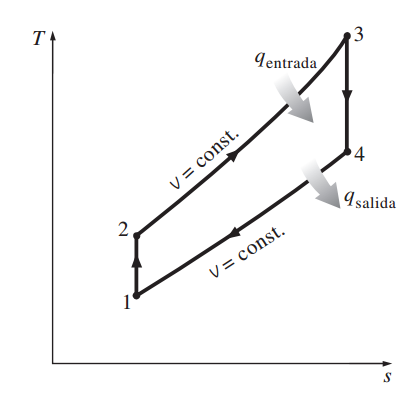
\includegraphics[width=0.5\textwidth]{Pasted_image_20250803093844.png}
        \caption{Ciclo de Otto ideal en diagrama T-s}
        \label{fig:otto_ts}
    \end{figure}

    \subsubsection{Eficiencia del Ciclo de Otto}

    Para un \textbf{sistema cerrado} bajo las \textbf{suposiciones de aire estándar frío}, la \hl{eficiencia térmica} del ciclo de Otto se deriva del \textbf{balance de energía}:

    \begin{equation}
    \eta_{Otto} = \frac{W_{neto}}{Q_H} = 1 - \frac{Q_L}{Q_H}
    \end{equation}

    Aplicando las \textbf{relaciones isentrópicas} y considerando que $v_2 = v_3$ y $v_4 = v_1$, se obtiene:

    \begin{equation}
    \eta_{Otto} = 1 - \frac{1}{r^{\gamma-1}}
    \end{equation}

    Donde:
    \begin{itemize}
        \item $r$: \hl{Relación de compresión} ($V_1/V_2$)
        \item $\gamma$: \textbf{Relación de calores específicos} ($c_p/c_v \approx 1.4$ para aire)
    \end{itemize}

    \begin{figure}[H]
        \centering
        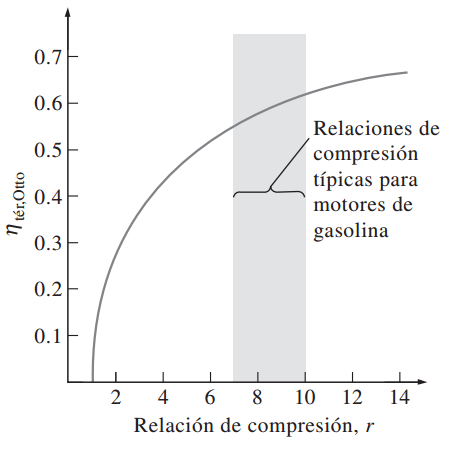
\includegraphics[width=0.6\textwidth]{Pasted_image_20250803100148.png}
        \caption{Eficiencia del ciclo Otto vs relación de compresión}
        \label{fig:eficiencia_otto}
    \end{figure}

    \subsection{El ciclo Diesel: motores de encendido por compresión}

    El \hl{ciclo Diesel}, también conocido como \textbf{ciclo de presión constante}, representa el \textbf{modelo termodinámico ideal} para los \textbf{motores de encendido por compresión}. La diferencia fundamental con el \hl{ciclo de Otto} radica en que la \textbf{adición de calor} (proceso de combustión) ocurre a \textbf{presión constante} en lugar de \textbf{volumen constante}.

    En los \textbf{motores diésel reales}, el \textbf{combustible} se inyecta directamente en el \textbf{aire comprimido} a alta temperatura, produciendo \textbf{autoignición} sin necesidad de \textbf{sistema de encendido} externo.

    \subsubsection{Procesos del ciclo Diesel ideal}

    El \textbf{ciclo Diesel ideal} consta de cuatro procesos:

    \paragraph{Proceso 1-2: Compresión Isentrópica}
    El \textbf{aire} (sin combustible) se comprime \textbf{adiabáticamente} desde el \textbf{PMI} hasta el \textbf{PMS}. Las \textbf{relaciones de compresión} en motores diésel son \textbf{significativamente mayores} que en motores Otto (típicamente \textbf{14:1 a 25:1}).

    \paragraph{Proceso 2-3: Adición de Calor a Presión Constante}
    Este proceso simula la \textbf{inyección y combustión} del combustible. Se añade calor ($Q_H$) al sistema manteniendo la \textbf{presión constante} mientras el \textbf{volumen aumenta}.

    \textbf{Calor añadido:}
    \begin{equation}
    Q_H = m c_p (T_3 - T_2)
    \end{equation}

    \textbf{Relación de corte:}
    \begin{equation}
    r_c = \frac{V_3}{V_2}
    \end{equation}

    \paragraph{Proceso 3-4: Expansión Isentrópica}
    Los \textbf{gases de combustión} se expanden \textbf{adiabáticamente}, generando el \textbf{trabajo de potencia}.

    \paragraph{Proceso 4-1: Rechazo de Calor a Volumen Constante}
    Simula la \textbf{expulsión} de gases de escape y \textbf{enfriamiento} del cilindro.

    \textbf{Calor rechazado:}
    \begin{equation}
    Q_L = m c_v (T_4 - T_1)
    \end{equation}

    \subsubsection{Eficiencia del Ciclo Diesel}

    La \hl{eficiencia térmica} del \hl{ciclo Diesel} bajo \textbf{suposiciones de aire estándar frío} se expresa como:

    \begin{equation}
    \eta_{Diesel} = 1 - \frac{1}{r^{\gamma-1}} \left[ \frac{r_c^{\gamma} - 1}{\gamma (r_c - 1)} \right]
    \end{equation}

    Donde:
    \begin{itemize}
        \item $r$: \hl{Relación de compresión} ($V_1/V_2$)
        \item $r_c$: \textbf{Relación de corte} ($V_3/V_2$)
        \item $\gamma$: \textbf{Relación de calores específicos}
    \end{itemize}

    \subsection{Comparación de ciclos y parámetros de rendimiento}

    La \textbf{comparación} entre los \textbf{ciclos termodinámicos ideales} nos permite comprender las \textbf{diferencias fundamentales} en el \textbf{diseño}, \textbf{operación} y \textbf{rendimiento} de los diferentes tipos de \textbf{motores de combustión interna}.

    \begin{table}[h]
    \centering
    \caption{Comparación de ciclos termodinámicos}
    \begin{tabular}{|l|l|l|l|}
    \hline
    \textbf{Característica} & \textbf{Ciclo de Otto} & \textbf{Ciclo Diesel} & \textbf{Ciclo de Carnot} \\
    \hline
    Tipo de Motor & Encendido por chispa & Encendido por compresión & Teórico ideal \\
    \hline
    Combustible & Gasolina, GLP & Diésel, biodiésel & Cualquier fluido \\
    \hline
    Ignición & Bujía de encendido & Autoignición & N/A \\
    \hline
    Adición de Calor & Volumen constante & Presión constante & Temperatura constante \\
    \hline
    Relación de Compresión & 8:1 a 12:1 & 14:1 a 25:1 & Variable \\
    \hline
    Eficiencia Típica & 25-30\% & 35-45\% & $\eta = 1 - T_L/T_H$ \\
    \hline
    \end{tabular}
    \label{tab:comparacion_ciclos}
    \end{table}

    \section{Ejercicios de Reforzamiento}

    \subsection{Ejercicio 1: Ciclo de Carnot}

    \textbf{Problema:} Una máquina térmica de Carnot opera entre una fuente térmica a 800 K y un sumidero a 300 K. Si recibe 1000 kJ de calor por ciclo, determine:
    \begin{enumerate}
        \item La eficiencia térmica del ciclo
        \item El trabajo neto producido por ciclo  
        \item El calor rechazado al sumidero
    \end{enumerate}

    \textbf{Solución:}

    a) \textbf{Eficiencia térmica:}
    \begin{equation}
    \eta_{Carnot} = 1 - \frac{T_L}{T_H} = 1 - \frac{300\text{ K}}{800\text{ K}} = 0.625 = 62.5\%
    \end{equation}

    b) \textbf{Trabajo neto:}
    \begin{equation}
    W_{neto} = \eta_{Carnot} \times Q_H = 0.625 \times 1000\text{ kJ} = 625\text{ kJ}
    \end{equation}

    c) \textbf{Calor rechazado:}
    \begin{equation}
    Q_L = Q_H - W_{neto} = 1000\text{ kJ} - 625\text{ kJ} = 375\text{ kJ}
    \end{equation}

    \subsection{Ejercicio 2: Ciclo de Otto}

    \textbf{Problema:} Un motor que opera según el ciclo de Otto tiene una relación de compresión de 10:1. Si $\gamma = 1.4$, determine:
    \begin{enumerate}
        \item La eficiencia térmica ideal del ciclo
        \item Compare con un motor de relación de compresión 8:1
    \end{enumerate}

    \textbf{Solución:}

    a) \textbf{Para r = 10:}
    \begin{equation}
    \eta_{Otto} = 1 - \frac{1}{r^{\gamma-1}} = 1 - \frac{1}{10^{1.4-1}} = 1 - \frac{1}{10^{0.4}} = 1 - 0.398 = 60.2\%
    \end{equation}

    b) \textbf{Para r = 8:}
    \begin{equation}
    \eta_{Otto} = 1 - \frac{1}{8^{0.4}} = 1 - 0.435 = 56.5\%
    \end{equation}

    \textbf{Conclusión:} El aumento de la relación de compresión de 8:1 a 10:1 mejora la eficiencia en 3.7 puntos porcentuales.

    \subsection{Ejercicio 3: Comparación Otto vs Diesel}

    \textbf{Problema:} Compare la eficiencia de un ciclo Otto (r = 9) con un ciclo Diesel (r = 18, $r_c = 2$) para $\gamma = 1.4$.

    \textbf{Solución:}

    \textbf{Ciclo Otto:}
    \begin{equation}
    \eta_{Otto} = 1 - \frac{1}{9^{0.4}} = 1 - 0.426 = 57.4\%
    \end{equation}

    \textbf{Ciclo Diesel:}
    \begin{equation}
    \eta_{Diesel} = 1 - \frac{1}{18^{0.4}} \left[ \frac{2^{1.4} - 1}{1.4(2-1)} \right] = 1 - 0.315 \times 1.171 = 63.1\%
    \end{equation}

    \textbf{Conclusión:} El ciclo Diesel muestra mayor eficiencia debido a su mayor relación de compresión.

    \section{Conclusión}

    Los \textbf{ciclos termodinámicos de potencia} estudiados constituyen la \textbf{base teórica fundamental} para comprender el funcionamiento de las \textbf{máquinas térmicas} utilizadas en \textbf{aplicaciones automotrices}. Aunque representan \textbf{idealizaciones} de los procesos reales, proporcionan \textbf{herramientas analíticas} esenciales para:

    \begin{enumerate}
        \item \textbf{Establecer límites teóricos} de rendimiento y eficiencia
        \item \textbf{Analizar} el comportamiento de \textbf{motores reales}
        \item \textbf{Identificar oportunidades} de mejora en el diseño
        \item \textbf{Comparar} diferentes \textbf{tecnologías} de motores
    \end{enumerate}

    El \hl{ciclo de Carnot} establece el \textbf{límite teórico superior} de eficiencia, sirviendo como \textbf{referencia} para evaluar el potencial de mejora de los ciclos reales. Los \textbf{ciclos de Otto y Diesel} representan los \textbf{fundamentos} de los motores de \textbf{encendido por chispa} y \textbf{encendido por compresión}, respectivamente.

    La \textbf{comprensión profunda} de estos conceptos es \textbf{crucial} para el \textbf{ingeniero automotriz} moderno, especialmente en el contexto actual de \textbf{transición energética} y \textbf{búsqueda de mayor eficiencia} en los \textbf{sistemas de propulsión vehicular}.

    \section{Bibliografía}

    Çengel, Y. A., \& Boles, M. A. (2015). \emph{Termodinámica} (8ª ed.). McGraw-Hill Education.

    Moran, M. J., Shapiro, H. N., Boettner, D. D., \& Bailey, M. B. (2018). \emph{Fundamentals of engineering thermodynamics} (9th ed.). John Wiley \& Sons.

    Payri, F., \& Desantes, J. M. (Coords.). (2011). \emph{Motores de combustión interna alternativos}. Editorial de la Universidad Politécnica de Valencia.

    Heywood, J. B. (2018). \emph{Internal combustion engine fundamentals} (2nd ed.). McGraw-Hill Education.

    Ferguson, C. R., \& Kirkpatrick, A. T. (2016). \emph{Internal combustion engines: Applied thermosciences} (3rd ed.). John Wiley \& Sons.

    Brunetti, F. (2012). \emph{Motores de combustión interna} (2ª ed.). Editorial Dossat.

    Pulkrabek, W. W. (2014). \emph{Engineering fundamentals of the internal combustion engine} (2nd ed.). Pearson.

\end{document}